\documentclass[../notes.tex]{subfiles}

\begin{document}

\section{Association Rules and Frequent Pattern Mining}
\subsection{The Frequent Pattern Mining Model}
\textbf{Basic Concepts:}
\begin{itemize}
\item Items $I = \{i_1, i_2, ..., i_m\}$, a set of literals 
\item Itemset $X$ (transaction): set of items $X \subseteq I$
\item Database $D$: set of transactions $T_i$ where $T_i \subseteq I$
\item $T$ contains $X$: $X \subseteq T$
\item Items in transactions or itemsets are sorted in lexicographic order
\item Length of itemset: number of elements of itemset
\item k-itemset: itemset of length $k$
\end{itemize}

\textbf{Supermarket example:}
\begin{itemize}
  \item Items $I = \{Bread, Butter, Milk, Eggs, Yogurt\}$ 
  \item Itemset $X$, Transaction $T$: 
    \begin{itemize}
      \item $X_1 = \{Bread, Butter\}$, $X_2 = \{Eggs, Milk\}$
      \item $T_1 = \{Bread, Butter, Milk\}$, $T_2 = \{Eggs, Milk, Yogurt\}$
    \end{itemize}
  \item Database $D$: set of transactions $T_i$ where $T_i \subseteq I$
    \begin{itemize}
      \item $T_1 = \{Bread, Butter, Milk\}$, $T_2 = \{Eggs, Milk, Yogurt\}$
      \item $D = \{T_1, T_2\} = \{\{Bread, Butter, Milk\}, \{Eggs, Milk, Yogurt\}\}$
    \end{itemize}
  \item $T$ contains $X$: $X \subseteq T$
    \begin{itemize}
      \item $X_1 = \{Bread, Butter\}$, $T_1 = \{Bread, Butter, Milk\}$
      \item $X_1 \subseteq T_1$
    \end{itemize}
  \item Items in transactions or itemsets are sorted in lexicographic order
  \item Length of itemset: number of elements of itemset
  \item k-itemset: itemset of length $k$
\end{itemize}

\textbf{Further Concept}
\begin{itemize}
  \item Support of itemset $X$ in $D$: percentage of transactions in $D$ containing $X$
    \begin{itemize}
      \item $sup(X, D) = \frac{|{T \in D | X \subseteq T}|}{|D|}$
    \end{itemize}
  \item Frequent itemset $X$ in $D$: item set X with
    \begin{itemize}
      \item $freq(X, D) :\Leftrightarrow sup(X, D) \ge minsup$
    \end{itemize}
  \item Association rule: implication of the form $ X \Rightarrow Y$
    \begin{itemize}
      \item where $X \subseteq I, Y \subseteq I$ and $X \cap Y = \varnothing$
    \end{itemize}
  \item Support $s$ of association rule $X \Rightarrow Y$ in $D$:
    \begin{itemize}
      \item indicates how frequently the itemset appears in the dataset
      \item support of $X \cup Y$ in $D$
      \item $s = \frac{|{T \in D | (X \cup Y) \subseteq T}|}{|D|}$
    \end{itemize}
  \item Confidence $c$ of association rule $X \Rightarrow Y$ in $D$:
    \begin{itemize}
      \item indicates how often the rule has been found to be true
      \item percentage of transactions containing $Y$ in the subset of all transactions in $D$ that contain $X$
      \item $c = \frac{|{T \in D | (X \cup Y) \subseteq T}|}{|{T \in D | X \subseteq T}|} = \frac{\sup(X \cup Y)}{\sup(X)}$
    \end{itemize}
\end{itemize}

\newpage

\subsection{Association Rules}
\subsubsection{Mining Association Rules}
1. Determine the frequent itemsets in the database \\
Naive algorithm: count the frequencies of all k-itemsets $\subseteq I$, inefficient since $\binom mk$ such itemsets \\

2. Generate the association rules from the frequent itemsets \\
Itemset $X$ frequent and $A \subseteq X$ \\
$A \Rightarrow (X-A)$ satisfies minimum support constraint (confidence remaining to be checked)

\subsubsection{Itemset Lattice}
\begin{itemize}
  \item Lattice: a partially ordered set with unique least upper bound and greatest lower bound.
  \item Itemset lattice:
    \begin{itemize}
      \item elements: itemsets $X_1 \subseteq I, X_2 \subseteq I, ..., X_n \subseteq I$
      \item partial order: $X_1 < X_2 :\Leftrightarrow X_1 \subset X_2$
      \item least upper bound: $I$
      \item greatest lower bound: $\varnothing$
    \end{itemize}
\end{itemize}

\begin{figure}[h]
\centering
\caption{Itemset Lattice}
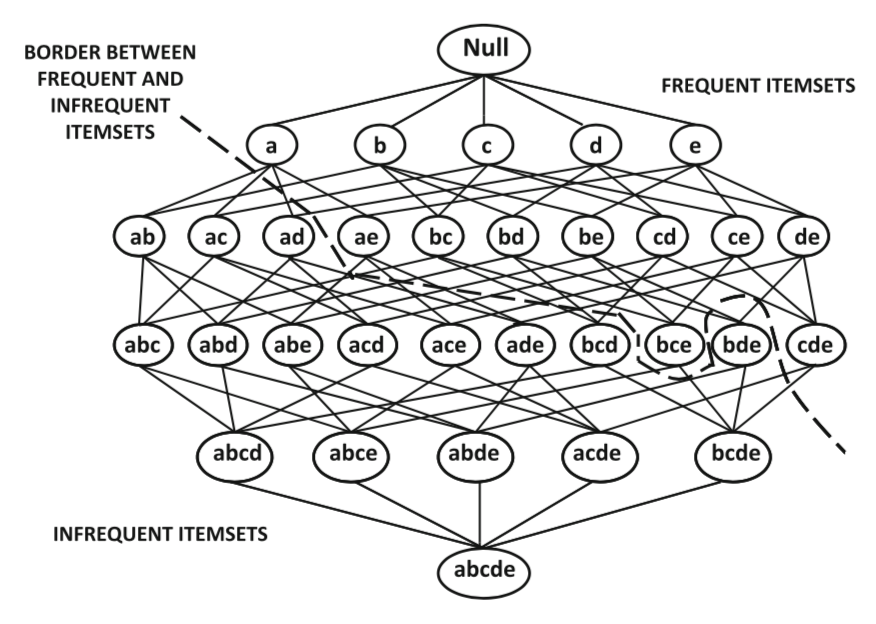
\includegraphics[width=7.5cm]{pic4-1}
\end{figure}

\subsubsection{Anti-monotonicity (downward closure) property}
Each subset of a frequent itemset is also frequent. \\
$\forall T_1 \subseteq I, T_2 \subseteq I: T_1 \subseteq T_2 \land freq(T_2, D) \Rightarrow freq(T_1, D)$ \\
because of \\
$\forall T_1 \subseteq I, T_2 \subseteq I: T_1 \subseteq T_2 \Rightarrow sup(T_1, D) \ge sup(T_2, D)$ \\

If one subset is not frequent, then superset cannot be frequent. \\
This property makes frequent itemset mining efficient, since in practice most itemsets are infrequent. 

\subsubsection{Computing the Association Rules}
\begin{itemize}
  \item Given a frequent itemset $X$
  \item For each subset $A$ of $X$, form the rule $A \Rightarrow (X - A)$
  \item Compute confidence of the rule $A \Rightarrow (X - A)$
    \begin{itemize}
      \item $confidence(A \Rightarrow (X - A)) = \frac{sup(X)}{sup(A)}$ 
    \end{itemize}
  \item Discard rules that do not have minimum confidence
  \item Store frequent itemsets with their supports in a hash table
    \begin{itemize}
      \item no DB acesses, no disk I/O
    \end{itemize}
\end{itemize}

\subsubsection{Interestingness of Association Rules}
\begin{itemize}
  \item Filter out misleading association rules
  \item Expected support for the rule $A \Rightarrow B$
    \begin{itemize}
      \item $P(A \cup B) = P(A) \cdot P(B)$
      \item assuming the idependence of A and B
    \end{itemize}
  \item Interestingness measure for rule $A \Rightarrow B$
    \begin{itemize}
      \item $\frac{P(A \cup B)}{P(A)} - P(B)$
      \item The larger this measure, the more interesting the discovered association between A and B
    \end{itemize}
  \item An alternative interestingness measure is the lift of an association rule
  \item If A and B are independent, then $P(A \cup B) = P(A) \cdot P(B)$
    \begin{itemize}
      \item i.e. $\frac{P(A \cup B)}{P(A) \cdot P(B)} = 1$
    \end{itemize}
  \item We define the lift of a rule $A \Rightarrow B$ as follows:
    \begin{itemize}
      \item $lift(A \Rightarrow B) = \frac{P(A \cup B)}{P(A) \cdot P(B)}$
      \item Can also be formulated as:
      \begin{itemize}
        \item $lift(A \Rightarrow B) = \frac{P(A \cup B) / P(A)}{P(B)} = \frac{support_{actual}}{support_{expected}}$
        \item as the ratio of the conditional probability $P(B|A)$ and the unconditional probability $P(B)$
      \end{itemize}
      \item A lift $>>1$ indicates that the discovered association between A and B is interesting.
    \end{itemize}  
\end{itemize}

\subsection{The Apriori Algorithm}
\subsubsection{Approach}
\begin{itemize}
  \item Determine first the frequent 1-itemsets, then frequent 2-itemsets, ...
  \item To determine the frequent k+1-items, consider only the k+1-items for which all k-subsets are frequent
  \item Calculation of support: one database scan counting the support for all relevant itemsets
\end{itemize}

\begin{algorithm}
\caption{Algorithm Apriori}
\begin{algorithmic}[0]
\State /* $C_k:$ set of candidate itemsets of length k */
\State /* $F_k:$ set of all frequent itemsets of length k */ \\
\Function{Apriori}{D, minsup}
\While{$F_k \ne \varnothing$}
  \State Generate $C_{k+1}$ by joining itemset-pairs in $F_k$;
  \State Prune itemsets from $C_{k+1}$ that violate anti-monotonicity;
  \State Determine $F_{k+1}$ by counting supoort of $C_{k+1}$ in D and retaining itemsets fron $C_{k+1}$ with support at least minsup;
  \State k = k + 1;
\EndWhile
\Return $\cup_k F_k$;
\EndFunction
\end{algorithmic}
\end{algorithm}

\newpage

\subsubsection{Candidate Generation}
Requirements for set $C_k$ of candidate itemsets
\begin{itemize}
  \item Superset of $F_k$
  \item Significantly smaller than set of all k-subsets of $I$
\end{itemize}

Step1: Join
\begin{itemize}
  \item Frequent k-1-itemsets $p$ and $q$, p and q are joined if they aggre in their first $k-2$ items
  \item E.g. $p \in F_{k-1} = \{1,2,3\}$, $q \in F_{k-1} = \{1,2,4\} \Rightarrow (1,2,3,4) \in C_k$
  \item Choose first k-2 items to avoid duplication without missing any candidates
\end{itemize}

Step2: Pruning
\begin{itemize}
  \item Remove all elements from $C_k$ having a k-1-subset not contained in $F_{k-1}$
  \item E.g. $F_3 = \{(1,2,3), (1,2,4), (1,3,4), (1,3,5), (2,3,4)\}$
  \item After join step: $C_4 = \{(1,2,3,4), (1,3,4,5)\}$
  \item In pruning step: remove $(1,3,4,5)$ since subsets $(1,4,5), (3,4,5)$ are missing
  \item $C_4 = \{(1,2,3,4)\}$
\end{itemize}

\subsubsection{Support Counting}
\textbf{for each} candidate $c \in c_k$ \textbf{do} c.count = 0; \\
\textbf{for each} transaction $T \in D$ \textbf{do} \\
\tab $CT := subset(C_k, T);$ // all candidates from $C_k$ that are contained in transaction $T$ \\
\tab \textbf{for each} candidate $c \in CT$ \textbf{do} c.count++; \\
$F_k := \{c \in C_k | (c.count / |D|) \ge minsup\}$\\

To achieve one scan over the database D, $subset(C_k, T)$ should be implemented properly. Thus we need Hash Tree.

\subsubsection{Hash Tree}
Hash tree as a data stucture for $C_k$
\begin{itemize}
  \item Leaf node: records list of itemsets (with frequencies)
  \item Inner node: contains hash table (apply hash function to d-th elements), each hash bucket at level $d$ references son node at level $d+1$
  \item Root has level 1
\end{itemize}

Finding an itemset
\begin{itemize}
  \item Start from the root
  \item At level $d$: apply hash function $h$ to the d-th element of the itemset.
\end{itemize}

Inserting an itemset 
\begin{itemize}
  \item Find the corrsponding leaf node and insert new itemset
  \item In case of overflow:
  \begin{itemize}
    \item Covert leaf node into inner node and create all its son nodes (new leaves).
    \item Distribute all entries over the new leaf nodes according to hash function $h$.
  \end{itemize}
\end{itemize}

\newpage

Find all candidates contained in $T = (t_1 t_2 t_3 ... t_m)$
\begin{itemize}
  \item At root
  \begin{itemize}
    \item Determine hash values $h(t_i)$ for each item $t_i$ in $T$
    \item Continue search in all correspoding son nodes
  \end{itemize}

  \item At inner node of level $d$
  \begin{itemize}
    \item Assumption: innder node has been reached by hashing $t_i$
    \item Determine hash values and continue search for all items $t_k$ in $T$ with $k > i$
  \end{itemize}

  \item At leaf node
  \begin{itemize}
    \item For each itemset $X$ in this node, test whether $X \subseteq T$
  \end{itemize}
\end{itemize}

\subsubsection{Methods of Efficiency Improvement}
\begin{itemize}
  \item Support counting using a hash table
  \begin{itemize}
    \item Hash table instad of hash tree, support counters for hash buckets
    \item k-itemset with correspoding bucket counter < minsup cannot be frequent
    \begin{itemize}
      \item more efficient access to candidates but inaccurate counts
    \end{itemize}
  \end{itemize}

  \item Reduction of transactions
  \begin{itemize}
    \item Transactions that do not contain any frequenct k-itemset are irrelevant
    \item Remove such transactions for future phases
    \begin{itemize}
      \item more efficient database scan, but additional writing of database
    \end{itemize}
  \end{itemize}

  \item Partitioning of the database
  \begin{itemize}
    \item Itemset is only frequent if frequent in at least one partition
    \item Form memory-resident partions of the database
    \begin{itemize}
      \item more efficient on partitions, but expensive combination of intermediate results
    \end{itemize}
  \end{itemize}

  \item Sampling
  \begin{itemize}
    \item Apply algorithm to sample to find frequent itemsets
    \item Count support of these frequent itemsets in the whole database
    \item Determine further candicates and support counting on the whole database
  \end{itemize}
\end{itemize}

\subsection{Enumeration-Tree Algorithms}
\begin{itemize}
  \item Frequent itemsets are stored in a tree-like data structure, the enumeration tree, which provides an abstract, hierarchical representation of the lattice of itemsets.
  \item Items within aset are ordered lexicographically (Lexicographic tree).
  \item Hierarchical structure supports systematic and non-redundant exploration of the lattice of itemsets. \\
  
  \item Nodes represent itemsets
  \item Edges represent subset relationships
  \item A child node $C = \{i_1, i_2, ..., i_k\}$ extends the parent node $P = \{i_1, i_2, ..., i_k-1\}$ by one item that is lexicographically larger than all items of the parent node
  \item The root represents the empty itemset (null)
\end{itemize}

\begin{figure}[h]
\centering
\caption{The lexicographic or enumeration tree of frequent itemsets}
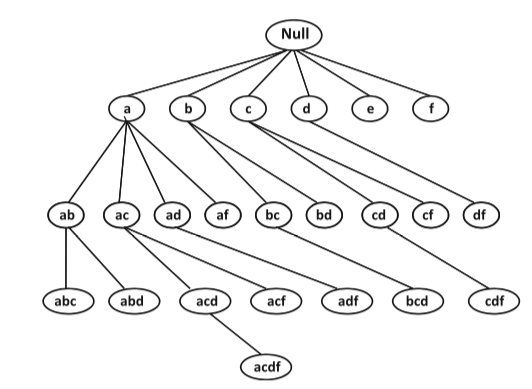
\includegraphics[width=6.2cm]{pic4-3}
\end{figure}

\begin{algorithm}
\caption{Generic Enumeration Tree}
\begin{algorithmic}[0]
\Function{GenericEnumerationTree}{D, minsup}
\State /* Initialize enumeration tree $ET$ to Null Node*/
\While{any node in $ET$ has not been examined}
  \State select one or more unexamined nodes $P$;
  \For {each $p$ in $P$}
    \State Generate candidate extensions $C(p)$;
  \EndFor
  \State Count support in $D$ for all $n$ in any $C(p)$;
  \If {support of n $\ge$ minsup}
    \State extend node $p$ by node $n$
  \EndIf
\EndWhile
\Return $ET$;
\EndFunction
\end{algorithmic}
\end{algorithm}

\subsubsection{Example Algorithms}
\begin{itemize}
  \item Apriori
    \begin{itemize}
    \item candidate generation is level-wise (breadth-first)
    \item joining siblings
    \item single databse scan to count support of all candidates of a level
    \end{itemize}
  \item FP-growth
    \begin{itemize}
    \item candidate generation is depth-first
    \item create projected databse of transactions supporting an itemset
    \item count support of candidate extensions only in projected database
      \begin{itemize}
        \item Minimize the number of candidate itemsets generated and counted, without missing any frequent itemsets
      \end{itemize}
    \end{itemize}
\end{itemize}

\subsection{Suffix-based Pattern Growth Methods}
\subsubsection{Recursive Suffix-based Pattern Growth}
\begin{itemize}
\item In Apriori, have to count support from scratch at every level
\item In order not to waste the computational effort of counting, form projected database for a frequent itemset P: all transactions containing itemset $P$
\item If a transaction does not contain the itemset corresponding to an enumeration-tree node, then this will not be relevant for counting at any descendent (superset itemset) of tht node.
\item Count support of extensions of P only in projected database of P.
\item Use absolute minsup, not relative minsup.
\item Start with empty pattern (suffix) and complete database $D$, where D has been filtered to contain only frequent items.
\item Recursive calls for all extensions and their projected databases.
\end{itemize}

\newpage

\begin{algorithm}
\caption{Algorithm Recursive Suffix Growth {\color{red} confusion waiting to be solved}}
\begin{algorithmic}[0]
\State /* D: transactions in terms of frequent 1-items, i.e. without infrequent items */
\State /* P: current suffix itemset */
\State /* reports all frequent itemsets with suffix $P$ */ \\

\Function{RecursiveSuffixGrowth}{D, minsup, P}
\For{\textbf{each} item \textbf{i} in any transaction of D}
  \State \textbf{report} itemset $P_i = \{i\} \cup P$  as frequent;
  \State Form $D_i$ with all transactions from $D$ containing item $i$;
  \State Remove all items from $D_i$ that are lexicographically $y \ge i$;
  \State Rmove all infrequent items from $D_i$
  \If{$D_i \ne \varnothing$}
    RecursiveSuffixGrowth($D_i, minsup, P_i$)
  \EndIf
\EndFor
\EndFunction
\end{algorithmic}
\end{algorithm}

\subsubsection{FP-Tree}
\begin{itemize}
  \item Space-efficient data structure for projected database
  \item Trie structure represents conditional database by consolidating the prefixes
  \item Path fron the root to a leaf represents a transaction (or a set of identical transactions)
  \item Path from the root to internal node represents a prefix of a transaction (or a transaction)
  \item Each node has count (in the original database) of transactions that support that prefix (or transaction)
  \item Prefixes are sorted in dictionary order
  \item Lexicographic ordering of items from most frequent to least frequent
  \begin{itemize}
    \item Maximizes the effect of prefix-based compression
      \begin{itemize}
        \item Item with a large support is more likely to be the prefix of many other itemsets
      \end{itemize}
    \item Balances the size of different conditional databases
  \end{itemize}
\end{itemize}

Construction of FP-Tree
\begin{itemize}
  \item Create an empty tree
  \item Remove infrequent items from the transactions
  \item Insert the modified transactions into the tree, one by one
  \item When the prefix of the transaction overlaps with an existing path, increment the counts of that path by 1
  \item For the non-overlapping part of the transaction, create new nodes with a count of 1. 
  \item If applicable, create pointer to ``next'' node with the same item
\end{itemize}

Extraction of conditional FP-Tree of item i
\begin{itemize}
  \item Chase pointers for item i to extract the tree of its conditional prefix paths. Prune remaining branches.
  \item Adjust counts in the prefix paths to account for the pruned branches
  \item Count frequency of each item by aggregating the counts of that item in the tree of prefix paths. Remove infrequent items. Item i is also removed.
    \begin{itemize}
      \item conditional FP-tree may have to be re-created by successive insertion of prefix paths
    \end{itemize}  
\end{itemize}

\subsection{Constraint-Based Association Mining}
\subsubsection{Motivation}
\begin{itemize}
  \item Too many frequent itemsets
    \begin{itemize}
      \item Mining is inefficient
    \end{itemize}
  \item Too many association rules
    \begin{itemize}
      \item hard to evaluate
    \end{itemize}  
  \item Constraints may be known apriori
    \begin{itemize}
      \item Constraints on the frequent itemsets
      \item e.g. ``association rules on product A but not on product B''
      \item e.g. ``only association rules with toal price $ > 100$''
    \end{itemize}  
\end{itemize}

\subsubsection{Types of constraints}
\begin{itemize}
  \item Domain Constraints
    \begin{itemize}
      \item $S \theta v, \theta \in \{=, \ne, <, \le, >, \ge\}$
      \begin{itemize}
        \item e.g. $S.price < 100$
      \end{itemize}

      \item $v \theta S, \theta \in \{\in, \notin\}$
      \begin{itemize}
        \item e.g. $snack \notin S.type$
      \end{itemize}

      \item $V \theta S$ or $S \theta V$, $\theta \in \{\subseteq, \subset, \not\subset, =, \ne\}$
      \begin{itemize}
        \item e.g. $\{snacks, wines\} \subseteq S.type$
      \end{itemize}
    \end{itemize}
  
  \item Aggregation Constraints
    \begin{itemize}
      \item $agg(S) \theta v$, where
      \begin{itemize}
        \item $agg \in \{min, max, sum, count, avg\}$
        \item $\theta \in \{=, \ne, <, \le, >, \ge\}$
      \end{itemize}
      \item $count(S_1.type) = 1, avg(S_2.price) > 100$
    \end{itemize}
\end{itemize}

\subsubsection{Application of the Constraints}
\begin{itemize}
  \item When determining the association rules
    \begin{itemize}
      \item Solves the evaluation problem
      \item But not the efficiency problem
    \end{itemize}
  \item When determining the frequent itemsets
    \begin{itemize}
      \item Can also solve the efficiency problem
      \item Challenge for candidate generation
    \end{itemize}
\end{itemize} 

\subsubsection{Anti-Monotonicity}
\begin{itemize}
  \item Definition: If an itemset $S$ violates an anti-monotone constraints $C$, then all supersets of $S$ violate this constraint.
  \item Examples
    \begin{itemize}
      \item $sum(S.price) \le v$ is anti-monotone
      \item $sum(S.price) \ge v$ is not anti-monotone
      \item $sum(S.price) = v$ is partly anti-monotone
    \end{itemize}
  \item Application
    \begin{itemize}
      \item Push anti-monotone constraints into candidate generation
    \end{itemize}
\end{itemize} 

\subsection{Multi-level Association Rules}
\subsubsection{Definitions}
\begin{itemize}
  \item $I = \{i_1, i_2, ..., i_m\}$ a set of literals (Items)
  \item $H$ a directed acyclic graph over $I$
  \item Edge in $H$ i to j:

  \begin{itemize}
    \item $i$ is a genralization of $j$
    \item $i$ is called $father$ or direct predecesor of $j$
    \item $j$ is a son or direct sucessor of $i$
  \end{itemize}

  \item $\bar{x}$ is predecessor of $x$ ($x$ successor of $\bar{x}$) w.r.t $H$:
  \begin{itemize}
    \item there is a path from $x$ to $x$ in $H$
  \end{itemize}

  \item Set of items $\bar{Z}$ is $predecessor$ of set items $Z$:
  \begin{itemize}
    \item at least one item in $\bar{Z}$ predecessor of an item in $Z$
  \end{itemize}

  \item $D$ is a set of transaction $T$, where $T \subseteq I$
  \item Typically, transactions $T$ contain only elements from the leaves of graph $H$
  
  \item Transaction $T$ supports item $i \in I$
  \begin{itemize}
    \item $i \in T$ or $i$ is predecessor of an item $j \in T$
  \end{itemize}
  
  \item $T$ supports set $X \subseteq I$ of items
  \begin{itemize}
    \item $T$ supports each item in $X$
  \end{itemize}

  \item Support of set $X \subseteq I$ of items in $D$
  \begin{itemize}
    \item Percentage of transactions in $D$ supporting X.
  \end{itemize}

  \item Multilevel association rule:
  \begin{itemize}
    \item $X \Rightarrow Y$ where $X \subseteq I, Y \subseteq I, X \cap T = \varnothing$
    \item and no item in Y is predecessor w.r.t. H of an item in X
  \end{itemize}

  \item Support $s$ of a multilevel association rule $X \Rightarrow Y$ in D:
  \begin{itemize}
    \item Support of set $X \cup Y$ in D
  \end{itemize}

  \item Confidence $c$ of a multilevel association rule $X \Rightarrow Y$ in D:
  \begin{itemize}
    \item Percentage of transactions containing $Y$ in the subset of all transactions in $D$ that contain $X$
  \end{itemize}
\end{itemize}

\newpage

\subsection{Determining the Frequent Itemsets}
\subsubsection{Idea}
\begin{itemize}
  \item Extend database transactions by all predecessors of items contained in that transaction

  \item Method
  \begin{itemize}
    \item Insert each item i transaction $T$ together with all its predessors w.r.t. $H$ into new transaction $T'$ 
    \item Do not insert duplicates
  \end{itemize}
 
  \item Then Determine frequent itemsets for basic association rules (e.g. Apriori algorithm)

  \item Basic algorithm for multilevel association rules
\end{itemize}

\subsubsection{Optimizations of the Basic Algorithm}
\begin{itemize}
  \item Materialization of Predecessors
  \begin{itemize}
    \item Additional data structure $H$: Item $\rightarrow$ list of all its predecessors
    \item More efficient access to the predecessors 
  \end{itemize}

  \item Filtering the predecessors to be added
  \begin{itemize}
    \item Add only those predecessors that occur in an element of candidate set $C_k$
    \item Example: $C_k = \{\{Clothes, Shoes\}\}$, replace ``JacketXT'' by ``Clothes''
  \end{itemize}

  \item Discard redundant item sets
  \begin{itemize}
    \item Let $X$ an k-item set, $i$ an item an $\bar{i}$ a predecessor of $i$
    \item $X = \{i, \bar{i}, ...\}$
    \item Support of $X - {i} = $ support of $X$
    \item X can be discarded during candidate generation
    \item Do not need to count supoort of k-itemset that contains item $i$ and predecessor of $i$
  \end{itemize} 

  \item Algorithm $Cumulate$
\end{itemize} 

\subsubsection{Stratification}
\begin{itemize}
  \item Alternative to the basic algorithm (Apriori-algorithm)
  \item Stratification = form layers in the candidates sets
  \item Property: Itemset $\bar{X}$ is infrequent and $\bar{X}$ is predecessor of $X$: $X$ is infrequent

  \item Method:
    \begin{itemize}
      \item Do not count all k-itemsets at the same time
      \item Count support first for the more general itemsets and cunt more special item serts only if necessary
    \end{itemize}

  \item Example:
   \begin{itemize}
      \item $C_k = \{\{Clothes, Shoes\}, \{Outerwear, Shoes\}, \{Jackets Shoes\}\}$
      \item Count support first for $\{Clothes, Shoes\}$
      \item Count support for $\{Outerwear, Shoes\}, \{Jackets Shoes\}\}$ only if $\{Clothes, Shoes\}$ is frequent
    \end{itemize}

  \item Notations
    \begin{itemize}
      \item $Depth$ of an itemset
        \begin{itemize}
          \item For itemsets $X$ in candidate set $C_k$ without direct predecessor in $C_k: Depth(X) = 0$
          \item For all other itemsets $X$ in $C_k$: \\ $Depth(X) = max\{Depth(\bar{X}) | \bar{X} \in C_k $ is direct predecessor of X\} + 1
        \end{itemize}
      \item $C_k^n:$ Set of itemsets from $C_k$ with depth $n$, $0 \le n \le$ maximal depth $t$
    \end{itemize} 

  \newpage

  \item Algorithm Stratify
  \begin{itemize}
    \item Count itemsets in $C_k^0$
    \item Remove all sucessors of infrequent element of $(C_k^0)$
    \item Count support for remaining elements of $C_k^1$
  \end{itemize}
  \item Trade-off between number of itemsets for which the support is counted (memory requirements) and the number of database scans (I/O cost)
  \item If $|C_k^n|$ is small, count candidates of depth $(n, n+1, ..., t)$ at the same time

  \item Problems of Stratify
  \begin{itemize}
    \item If many itemsets of small depth are frequent
    \item Can discard only few itemsets of larger depths
  \end{itemize}

  \item Improvements of Stratify
  \begin{itemize}
    \item Estimate support of all itemsets in $C_k$ using a sample.
    \item $C_k':$ all itemsets which have estimated supoort exceeding minimum support.
    \item Determine actual support of all itemsets in $C_k'$ in one database scan.
    \item Removve all successors of infrequent elements of $C_k'$ to form $C_k''$
    \begin{itemize} 
      \item $C_k'' = C_k - C_k'$
    \end{itemize}
    \item Determine support for the remaining elements of $C_k''$ in a second database scan
  \end{itemize}
\end{itemize}

\subsection{Interestingness of Multilevel Association Rules}
\begin{itemize}
  \item $\bar{X} \Rightarrow \bar{Y}$ is predecessor of $X \Rightarrow Y$ \\ 
  Itemsets $\bar{X}$ is predecessor of item set $X$ and/or item set $\bar{Y}$ is predecessor of set $Y$

  \item $\bar{X} \Rightarrow \bar{Y}$ direct predecessor of $X \Rightarrow Y$ in a set of rules: \\
  $\bar{X} \Rightarrow \bar{Y}$ is predecessor of $X \Rightarrow Y$, and there is no rule $X' \Rightarrow Y'$ \\
  such that $X' \Rightarrow Y'$ predecessor of $X \Rightarrow Y$ and $\bar{X} \Rightarrow \bar{Y}$ predecessor of $X' \Rightarrow Y'$

  \item Multilevel association rule $X \Rightarrow Y$is R-interesting
  \begin{itemize} 
    \item Has no direct predecessors $or$
    \item Actual support (confidence) $ > R$ times the expected support (confidence)
    \item And the direct predecessor is also R-interesting
  \end{itemize}

\end{itemize}

\subsection{Multilevel Association Rules}
Choice of $minsup$
\begin{itemize} 
  \item Fix support
  \begin{itemize} 
    \item Same $minsup$ value for all levels of the item taxonomy
    \item + Efficiency: pruning successors of in frequent itemsets
    \item - Reduced effectiveness
    \begin{itemize} 
      \item $minsup$ too high $\Rightarrow$ no low-level associations 
      \item $minsup$ too low $\Rightarrow$ too many high-level associations
    \end{itemize}
  \end{itemize}

  \item Variable support
  \begin{itemize} 
    \item Different $minsup$ values for different levels of the item taxonomy
    \item + Good effectiveness: find association rules at appropriate support level
    \item - Inefficient: no pruning of successors of infrequent itemsets
  \end{itemize}
\end{itemize}
\newpage

\subsection{Pattern Summarization}
\subsubsection{Overview}
\begin{itemize} 
  \item In many applications, there are too many frequent itemsets (patterns).
  \item Leads to inefficient mining.
  \item Makes it hard for user to analyze the patterns in a meaningful way
  \item The vast majority of the generated patterns are typically redundant.
  \item Thus, we need to summarize sets of patterns \\

  \item Closed frequent itemsets
  \begin{itemize} 
    \item lossless compression: can reconstruct all frequent itemsets and their support
  \end{itemize}

  \item Maximal frequent itemsets
  \begin{itemize} 
    \item lossy compression: can reconstruct all frequent itemsets but not their support
  \end{itemize}

  \item Approximate representations
  \begin{itemize} 
    \item lossless compression: can reconstruct neither all frequent itemsets nor their support
  \end{itemize}
\end{itemize}

\subsubsection{Closed Frequent Itemsets}
\begin{itemize} 
  \item An itemset $X$ is closed, if none of its supersets has the same support as $X$
  \item S(X): set of subset of X, which have the same support as $X$
  \item Every itemset in $S(X)$ is supported by the same set of transactions, and therefore, it suffices to keep $X$ as the single representative itemset. 
  \item Goal is to produce all closed, frequent itemsets.
  \item Two approaches:
  \begin{itemize} 
    \item post-process the results of frequent itemset mining
    \item directly find the closed frequent patterns during the process of frequent pattern discovery
  \end{itemize}
\end{itemize}

\subsubsection{Mining Closed Frequent Itemsets}
\begin{itemize} 
  \item Partition the set $F$ of frequent itemsets into equi-support groups.
  \item The maximal itemsets from each equi-support group are closed frequent itemsets and are to be determined
  \item For that goal, the pattern in an equi-support group are processed in decreasing order of length and either ruled in or ruled out, depending on whether or not they are closed.
  \item This order ensures that closed patterns are encountered before their redundant subsets
  \item Initially, all patterns are unmarked
  \item When an unmarked pattern $X \in F$ is processed, it is added to the frequent closed set $CF$.
  \item The proper subsets of $X$ with the same support are marked. To achieve this goal, the subset of the itemset lattice representing $F$ can be traversed in depth-first or breadth-first order starting at $X$, and exploring subsets of $X$. Itemsets that are subsets of $X$ are marked when thet have the same support as $X$.
  \item The traversal process backtracks when an itemset is reached with strictly larger support, or the itemset has already been marked.
  \item After the traversal is complete, the next unmarked node is selcted for further exploration and added to CF.
\end{itemize}

\subsubsection{Maximal Frequent Itemsets}
\begin{itemize} 
  \item A frequent $X$ is maximal, if none of its supersets is frequent.
  \item Maximal frequent itemsets are closed.
  \item The number of maximal frequent itemsets may be orders of magnitude smaller than the number of all frequent itemsets
  \item Naive algorithm: determine all frequent itemsets, and post-process them to remove all non-maximal ones.
  \item Direct algorithm: most tree-enumeration algorithms can be modified with the concept of look-aheads to directly determine only (mostly) maximal patterns.
\end{itemize}

\subsubsection{Naive Algorithm}
\begin{itemize} 
  \item Apply any algorithm to determine all frequent itemsets.
  \item Examine itemsets in decreasing order of length, removing all proper subsets of a given itemset.
  \item Continue until all itemsets have either been examined or have been removed.
  \item The itemsets that have not been removed at termination are the maximal ones.
\end{itemize}

\subsubsection{Direct Algorithm}
\begin{itemize} 
  \item Let C(P) be the set of candidate extenstions of node (frequent itemset) P
  \item Before support couting, test whether $P \cup C(P)$ is subset of a frequent pattern that has already been found.
  \item If yes, $P \cup C(P)$ is non-maximal frequent pattern, and the entire subtree (of the enumeration tree) rooted at $P$ can pruned.
  \item If $P$ cannot be pruned, the supports its support of its candidate extensions need to be determined. During this support counting, the support of $P \cup C(P)$ is counted along with the individual item extensions of P.
  \item If $P \cup C(P)$ is frequent, then it eliminates any further work of counting the supprt of nodes in the subtree rooted at node $P$.
  \item This subset-based pruning approach is particularly effecive with depth-first methods.
  \item Maximal patterns are found much earlier with a depth-first strategy than with a breadth-first strategy.
  \item For a maximal pattern of length $k$, the depth-first approach discovers it after exploring only (k-1) of its prefixs, rather than the $2^k$ subsets. This maximal pattern then becomes available for subset-based pruning.
  \item The pruning approach provides a smaller set of patterns that includes all maximal pattern but may also include some non-maximal pattern despite pruning.
\end{itemize}

\end{document}